
%\documentclass[calculator,datasheet,solutions]{exam}
\documentclass[calculator,datasheet]{exam}

% The full list of class options are
% calculator : Allows approved calculator use.
% datasheet : Adds a note that data sheet are attached to the exam.
% handbook : Allows the use of the engineering handbook.
% resit : Adds the resit markings to the paper.
% sample : Adds conspicuous SAMPLE markings to the paper
% solutions : Uses the contents of \solution commands (and \solmarks) to generate a solution file

\usepackage{pdfpages}
\usepackage{lscape,comment}

\coursecode{EG5597}%%
\coursetitle{Advanced Chemical Engineering}%
%\coursecode{EG3539}% 
%\coursetitle{Thermodynamics}%

\examtime{00.00--00.00}%
\examdate{00}{05}{2015}%
\examformat{Candidates must attempt \textit{all} questions.}

\newcommand{\frc}{\displaystyle\frac}
\newcommand{\br}[1]{\!\left( #1 \right)}
\newcommand{\abs}[1]{\left| #1 \right|}
\newcommand{\fracd}[2]{\frac{\mathrm{d} #1}{\mathrm{d} #2}}
\newcommand{\fracp}[2]{\frac{\partial #1}{\partial #2}}
\renewcommand{\d}[1]{\mathrm{d} #1 }
\newcommand{\Ma}{\mathrm{M\!a}}



\begin{document}

%%%
%%% QUESTION 1
%%%
\begin{question}

Answer all of the following questions.

\begin{enumerate}[(a)]
%
\item Consider the closed-loop block diagram of the process given below. Investigate the effect of a (a $>$ 0) on the stability of the system applying the Routh-Hurwitz stability criterion. K$_{c}$ can be positive or negative.~\marks{8}
\begin{center}
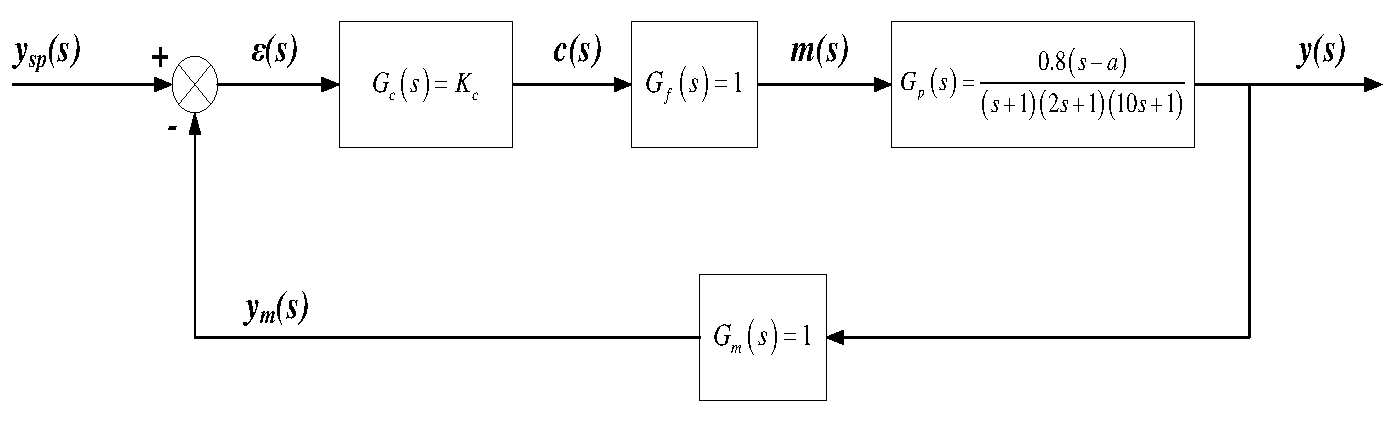
\includegraphics[width=\columnwidth]{./Pics/EG5597_Control_1_May_2014-5.pdf}
\end{center} 
\item Construct the Root-Locus of the closed-loop control system with the following open-loop transfer function, applying the 7 rules for Root-Locus definition. The Root-Locus should be qualitative, but correct on all structural features.~\marks{12}
\begin{displaymath}
G(s) = \frc{K(s+3)}{s(s+2)(s+4)}  
\end{displaymath}
\end{enumerate}

\underline{Useful equations}:
\begin{itemize}
\item Asymptotes angles with positive direction of {\it Re}-axis: 
\begin{displaymath}
\varphi_{i} = \frc{2k + 1}{n -m}\pi,\;\;\;k=0,\cdots,n-m-1
\end{displaymath}

\item Asymptotes centre of gravity:
\begin{displaymath}
\gamma=\frc{\left[\sum\limits_{i=1}^{n}p_{i}-\sum\limits_{j=1}^{m}z_{i}\right]}{(n-m)}
\end{displaymath}

\item Departure/arrival points of branches: 
\begin{displaymath}
\sum\limits_{i=1}^{n}\frc{1}{\left(s_{0}-p_{i}\right)}=\sum\limits_{j=1}^{m}\frc{1}{\left(s_{0}-z_{j}\right)}
\end{displaymath} 

\end{itemize}

\end{question}

\clearpage

%%%
%%% Question 02 
%%%
\begin{question}
%
Consider the following transfer function, where K$_{p}$=1,
\begin{displaymath}
G(s) = \frc{K_{p}}{(100s+1)(10s+1)(s+1)}
\end{displaymath}
\begin{enumerate}[(a)]
\item Construct the pair of Bode diagrams (amplitude and phase lag) for the above function. Graphs should be qualitative, but correct on all structural features.~\marks{13}

\item Construct the Nyquist plot for the above function. Plot should be qualitative, but correct on all structural features.~\marks{7}
\end{enumerate} 

\underline{Useful equations}:\\
	For a generic first-order system with transfer function $G_{x}(s)=\frc{K_{p}}{\tau_{p}s+1}$ under sinusoidal input of frequency $\omega$, the amplitude ratio of the output is $AR_{x}=\frc{K_{p}}{\sqrt{1+\tau_{p}^{2}\omega^{2}}}$ and the phase lag is $\varphi_{x}=\tan^{-1}\left(-\tau_{p}\omega\right)$


%
\end{question}

\clearpage


%%%%%%%%%%%%%%%%%%%%%%%%%
%%% Question 03       %%% 
%%%%%%%%%%%%%%%%%%%%%%%%%
\begin{question} 

The following oil, gas, water separation arrangement is proposed for an offshore development. It is a single process train comprising two stages of three phase separation with interstage heating. An export pump and cooler deliver the oil to an export pipeline. The export pump is driven by a fixed speed electric motor in a 2 x 100$\%$ parallel configuration. Large quantities of water are produced from each separator and the water is treated prior to overboard disposal. The inter-stage heater is an electric unit. Electrical supply is from a simple cycle, gas turbine coupled to a generator -– the gas turbine is powered by process gas. The system is designed for a 100$\%$ throughput but as the development ages, flow rates will drop progressively to 10$\%$ of design.  The initial discharge requirement from the pump is 100 bar, but as the throughput reduces the back pressure from the pipeline reduces requiring less pump discharge pressure.

Review the arrangement, identify and describe examples of energy saving opportunities. Key pressures and temperatures are indicated.~\marks{20}
\begin{center}
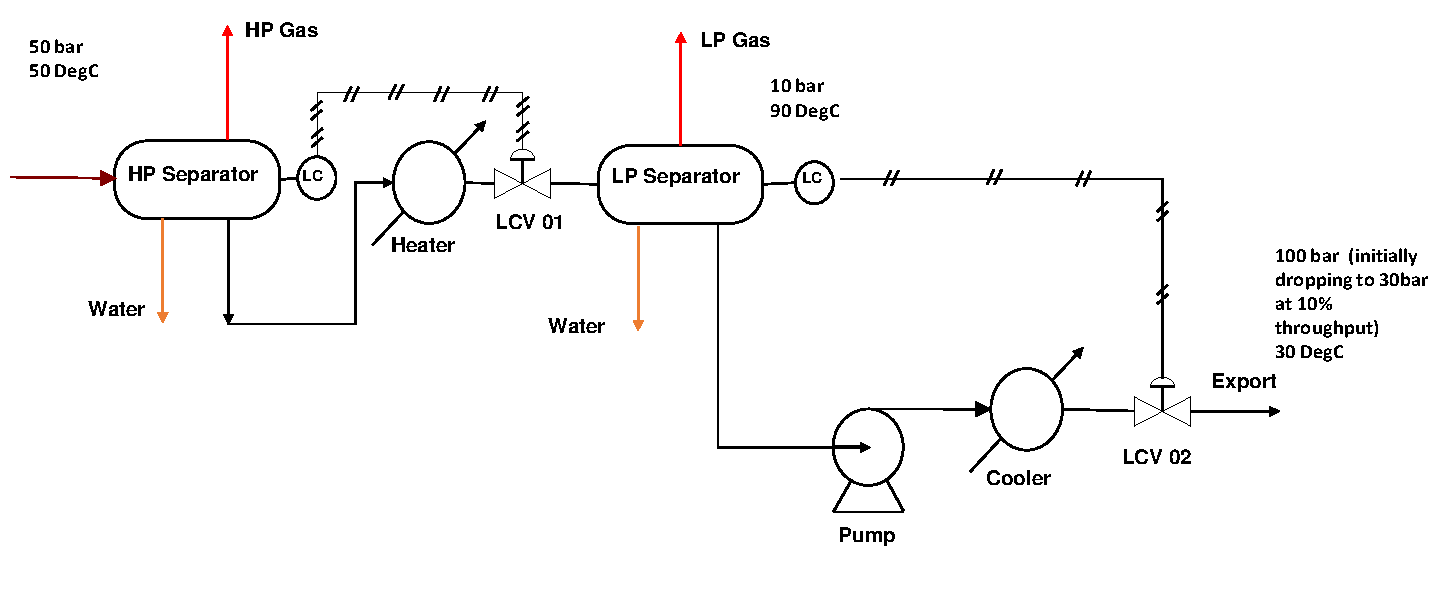
\includegraphics[width=\columnwidth]{./Pics/EG5597_Process_1_May_2014-5.pdf}
\end{center} 


\end{question}

\clearpage


%%%%%%%%%%%%%%%%%%%%%%%%%
%%% Question 04       %%%
%%%%%%%%%%%%%%%%%%%%%%%%%
\begin{question} 
Radioisotopes are often used in industrial facilities to assess the mechanical integrity (e.g., existence of micro-fractures) of equipment and pipeline network system. A prescribed quantity of isotopes is diluted in an inert solvent $\left(\rho=\text{877.15 kg.m}^{-3}\right)$ and is continuously injected at constant mass flow rate of 200 kg.s$^{-1}$ into a pipe of 0.762 of diameter and 6.5 meters of length.  In order to better analyse the data, a system engineer needs to calculate the expected distribution of radioisotopes throughout the pipe during the first 30 seconds of the test-injection. She decides to represent the concentration of radioisotopes, $\mathcal{C}\left(x,t\right)$ $\left(\text{in }\mu\text{g.m}^{-3}\right)$, as a 1D problem using a forward discretisation scheme in space and time (FDM) resulting in,
\begin{displaymath}
\mathcal{C}_{i}^{j+1}=\mathcal{C}_{i}^{j} - \frac{u\Delta t}{\Delta x }\left(\mathcal{C}_{i+1}^{j}-\mathcal{C}_{i}^{j}\right)
\end{displaymath}
where $i\in\left\{1,2,...,N_{x}\right\}$ and $j\in\left\{1,...,N_{t}\right\}$ are spatial- and time-increment indexes, respectively. She assumed:
\begin{itemize}
\item The domain is divided into $N_{x}=5$ nodes;
\item Time step size $\left(\Delta\text{t}\right)$ of 0.5 seconds;
\item Initial condition $\left(\text{in }\mu\text{g.m}^{-3}\right)$ is given by,
\[
\mathcal{C}\left(x,t=0\right)=
\left\{\begin{array}{l l}
\displaystyle\frac{2.0}{1.0 + e^{0.9\left(x-5.\right)}}  & \text{ for }  x \le 5.0 \text{ m }\\
1.0 & \text{ elsewhere.}
\end{array}\right.\]
\item {\it Ghost-node}: $x_{N_{x}+1}=x_{N_{x}}$
\item Dirichlet boundary condition: $\mathcal{C}\left(x=0,t\right)$=0.15 $\mu$g.m$^{-3}$
\end{itemize}
\begin{enumerate}[(a)]
\item Calculate the concentration profile of the radioisotope at t = 1.5 seconds, i.e., $\mathcal{C}_{i}^{j}$ $\forall i$ and $j=3$;~\marks{12} 
\item At t = 1s, the observed concentration (obtained from non-invasive sensor measurements) was:
\begin{displaymath}
\mathcal{C}^{\text{obs}}\left(x,t=1s\right)= \left(0.16 \;\; 2.00 \;\; 2.01 \;\; 1.15 \;\; 1.31\right)^{T}
\end{displaymath}
The sensors were placed in the same coordinates as the original simulated mesh grid. How would the engineer quantitatively assess the accuracy of her simulated data with respect to the measurements?~\marks{8} 
\end{enumerate}

\end{question}

\clearpage

%%%%%%%%%%%%%%%%%%%%%%%%%
%%% Question 05       %%%
%%%%%%%%%%%%%%%%%%%%%%%%%
\begin{question}
Polyisobutenyl succinic anhydride (PIBSA) is an ExxonMobil patented product used in oil additives to enhance the thermo-mechanical performance of engines. Initially polyisobutene monomer (PIB) is diluted in light mineral oil (in a stirred and jacketed reactor) and chlorinated at 200$^{\circ}$C. $Cl_{2}$ gas is injected from the bottom of reactor at a prescribed mass flow rate. After the chlorination, maleic anhydride (MalAnh)  is added into the vessel for the reaction at 250$^{\circ}$C and atmospheric pressure, releasing chlorine gas,
\begin{eqnarray}
 PIB \text{ (l)} + Cl_{2} \text{ (g)} &\Longleftrightarrow& Cl \cdot PIB \cdot Cl \text{ (l)} + H_{2} \text{ (g)}\nonumber \\
 Cl \cdot PIB \cdot Cl \text{ (l)} + H_{2} \text{ (g)} + MalAnh &\Longleftrightarrow& PIBSA \text{ (l)} + Cl_{2} \text{ (g)} + H_{2} \text{ (g)} \nonumber 
\end{eqnarray}
Fluid mixing and heat transfer are key aspects in the design and control of this process, therefore 4 baffles, mechanical stirrer, external heat-jacket and continuous $Cl_{2}$ gas injection are included in the system. Key-variables for modelling this system are (spatial and temporal): velocities $\left[{\bf u}\left(\underline{x},t\right)\right]$, pressure $\left[P\left(\underline{x},t\right)\right]$, temperature $\left[T\left(\underline{x},t\right)\right]$ and concentration of species $\left[\mathcal{C}_{i}\left(\underline{x},t\right)\right]$ (where $i\in\left\{1,2,\cdots\right\}$ corresponds to the different chemical species in solution). Describe the mathematical and physical formulations for the problem with all the necessary assumptions. This must include all steps from the initial formulation, and pre-processing to the beginning of the simulation. Given the conservative equations:~\marks{20}
\begin{itemize}
\item Conservation of mass:
\begin{displaymath}
\frc{\partial}{\partial t}\left(\rho_{i}\alpha_{i}\right) + \nabla\cdot\left(\rho_{i}\alpha_{i}\mathbf{u}_{i}\right)=\mathcal{S}_{\text{cty},i}
\end{displaymath}
where $\alpha_{i}$ is the volume fraction of phase $i$ (gas or liquid) and $\mathcal{S}_{\text{cty},i}$ is a source term for the continuity equation.

\item Conservation of momentum:
\begin{displaymath}
\frc{\partial}{\partial t}\left(\rho_{i}\alpha_{i}\mathbf{u}_{i}\right) + \nabla\cdot\left(\rho_{i}\alpha_{i}\mathbf{u}_{i}\mathbf{u}_{i}\right) = -\alpha_{i}\nabla P_{i} + \alpha_{i}\rho_{i}\mathbf{g} + \nabla\underline{\underline{\tau}} +\beta\left(\mathbf{u}_{i}-\mathbf{u}_{j}\right) + \Gamma_{i}\mathbf{u}_{i} + \mathcal{S}_{\text{mom},i}
\end{displaymath}
where $\beta$, $\underline{\underline{\tau}}$ and $\Gamma$ are the iterphase momentum transfer (drag) coefficient, stress tensor, gravity body force and frictional forces between suurfaces and fluid$i$, respectively. 

\item Conservation of thermal energy:
\begin{eqnarray}
\frc{\partial}{\partial t}\left(\rho_{i}\alpha_{i}\mathbf{u}_{i}C_{p,i}T_{i}\right) + \nabla\cdot\left(\rho_{i}\alpha_{i}C_{p,i}T_{i}\mathbf{u}_{i}\right) &=& -P_{i}\nabla\left(\alpha_{i}\mathbf{u}_{i}\right) + \nabla\left(\alpha_{i}\kappa_{i}\nabla T_{i}\right) + \nonumber \\
&& \gamma_{i}\left(T_{i}-T_{j}\right) + \Omega_{w,i} + \mathcal{S}_{\text{therm},i} \nonumber
\end{eqnarray}
where $C_{p}$, $\kappa$, $\gamma$ and $\Omega$ are heat capacity at constant pressure, thermal diffusivity, interphase heat transfer coefficient and the wall-phase heat transfer, respectively.

\item Conservation of species
\begin{displaymath}
\frc{\partial}{\partial t}\left(\rho_{i,j}\omega_{i,j}\right) + \nabla\cdot\left(\rho_{i,j}\omega_{i,j} \mathbf{u}_{i}\right) = \nabla\cdot\left(\rho_{i,j}D_{eff,i,j}\nabla\omega_{i,j}\right) + \mathcal{R}_{i,j}
\end{displaymath}
where $i$ and $j$ are indices for phase (liquid or gas) and chemical species, respectively. $D_{eff}$, $\omega$ and $\mathcal{R}$ are the effective mass diffusivity, mass fraction and reaction rate, respectively.

\end{itemize}

\end{question}


\vfill


\paperend


\end{document}
